%Version 3.1 December 2024
% See section 11 of the User Manual for version history
%
%%%%%%%%%%%%%%%%%%%%%%%%%%%%%%%%%%%%%%%%%%%%%%%%%%%%%%%%%%%%%%%%%%%%%%
%%                                                                 %%
%% Please do not use \input{...} to include other tex files.       %%
%% Submit your LaTeX manuscript as one .tex document.              %%
%%                                                                 %%
%% All additional figures and files should be attached             %%
%% separately and not embedded in the \TeX\ document itself.       %%
%%                                                                 %%
%%%%%%%%%%%%%%%%%%%%%%%%%%%%%%%%%%%%%%%%%%%%%%%%%%%%%%%%%%%%%%%%%%%%%
\documentclass[pdflatex,sn-mathphys-num]{sn-jnl}% Math and Physical Sciences Numbered Reference Style
%%%% Standard Packages
\usepackage{graphicx}%
\usepackage{multirow}%
\usepackage{amsmath,amssymb,amsfonts}%
\usepackage{amsthm}%
\usepackage{mathrsfs}%
\usepackage[title]{appendix}%
\usepackage{xcolor}%
\usepackage{textcomp}%
\usepackage{manyfoot}%
\usepackage{booktabs}%
\usepackage{algorithm}%
\usepackage{algorithmicx}%
\usepackage{algpseudocode}%
\usepackage{listings}%
\setlength{\parindent}{20pt}

\theoremstyle{thmstyleone}%
\newtheorem{theorem}{Theorem}%
\newtheorem{proposition}[theorem]{Proposition}%
\theoremstyle{thmstyletwo}%
\newtheorem{example}{Example}%
\newtheorem{remark}{Remark}%
\theoremstyle{thmstylethree}%
\newtheorem{definition}{Definition}%
\raggedbottom

\begin{document}

\title[Article Title]{Are taxi rides just a game? Analyzing taxi tipping behavior between drivers and passengers}

\author[]{\fnm{Julia} \sur{Fausto}}\email{julia.beatriz.v.fausto.26@dartmouth.edu}
\author[]{\fnm{Lourdes} \sur{Lauterborn}}\email{lourdes.b.lauterborn.28@dartmouth.edu}
\author[]{\fnm{Charles} \sur{Nelson}}\email{charles.t.nelson.29@dartmouth.edu}
\author[]{\fnm{Mithun} \sur{Rameshkumar}}\email{mithun.rameshkumar.28@dartmouth.edu}

\affil[]{\orgdiv{Department of Mathematics, Math 30.04 (Evolutionary Game Theory)},
\orgname{Dartmouth College},
\orgaddress{\city{Hanover},
\postcode{03755},
\state{NH},
\country{USA}}}

\abstract{Taxi tipping in New York City involves a strategic interaction with partially misaligned incentives. Drivers can maximize earnings either by providing efficient service in exchange for a tip (Tip-Max) or by extending trips to inflate the meter fare (Meter-Max), while passengers can choose to tip or not. We model this dyad as a two-population asymmetric game and analyze its dynamics with replicator dynamics, calibrated to approximately 6.5~million credit-card-paid Manhattan rush-hour rides drawn from the NYC Taxi \& Limousine Commission trip records across 13 quarters spanning February 2023 through February 2026. The model produces two analytical results. First, the cooperative outcome, which are Tip-Max drivers and tipping passengers, is never evolutionarily stable, as meter-maxing strictly dominates tip-maxing for drivers because the meter premium $m$ enters the fitness difference as a constant additive advantage, independent of passenger behavior. Second, the system exhibits a phase transition at $(\alpha + \beta)\ln(n) = \tau$. When social signaling exceeds the tip cost, the system equilibrates at $(0, 1)$. This means all-meter-max drivers, all-tipping passengers and is sustained by reputational incentives alone; otherwise the system collapses to $(0, 0)$. Empirically, the meter-max premium $m$ exceeds the mean tip $\tau$ in every quarter, NYC's credit-card tip incidence holds near 95\%, and the January 2025 NYC congestion fee---which compressed discretionary meter-padding---coincided with a +1.28~percentage-point jump in the mean tip rate. We interpret NYC's tipping equilibrium as norm-sustained rather than reciprocity-driven, with practical implications for transportation policy design.}

\keywords{evolutionary game theory, replicator dynamics, tipping behavior, taxi service, NYC TLC data, indirect reciprocity}

\maketitle

\section{Introduction}\label{sec1}
Every taxi ride can be seen as a small game. Drivers and riders have individual incentives, which establish various strategic interactions between the two parties. Considering yellow cabs with ticking meters, drivers want to maximize their earnings. They can do that in two ways: drive efficiently and earn a tip, or take longer and run up the meter. On the passenger side, their payoff structure runs in the opposite direction as they want to keep their costs down. A faster trip with a more direct route reduces both the meter fare and the time cost of being in the cab for passengers. Passengers decide between tipping and not tipping, given social norms and pressures of tipping. Passengers who tip give up some money but enjoy reputational benefits from being seen as generous, particularly when riding with other passengers who observe the transaction. It is important to remember that tipping is completely voluntary. This tension of partially aligned incentives is core to what this paper explores, and analyzing this matters because the outcome is not just about a few dollars. It also has direct welfare and economic implications: inefficient routing can have several effects, from congestion to an increase in travel time and to costs in an already overburdened urban environment, while also affecting driver income and broader social norms.

Our project explores the cab scene in New York City and analyzes how the strategic interactions between drivers and passengers play out through an evolutionary game theory lens and real ride data. Questions we grapple with are: Does the cooperative norm of drivers driving efficiently and passengers tipping survive? Does this equilibrium collapse under individual incentives or depend on third-party nudges? To answer these questions, we utilize replicator dynamic models to evaluate how strategic incentives respond to each other in the rush hour scene of Manhattan. We therefore restrict our analysis to 6.5~million credit-card Yellow Taxi trips in Manhattan during weekday rush hours, using data from the NYC Taxi \& Limousine Commission's public trip records~\cite{tlc2024}.

Prior work on tipping has framed our approach. Norris et al.~\cite{norris2023} applied static game theory to restaurant tipping, finding that service quality and group size are recognized as factors influencing the customer's decision-making on tipping amount. This finding informs our model assumptions by suggesting that observable service characteristics affect tipping through social signaling rather than pure reciprocity, which motivates our use of group size as a relevant observable characteristic in our context. Kang~\cite{kang2021} argued that tipping in service industries is sustained by social norms. Even when their underlying economic incentives shift, people continue to tip out of habit and pressure rather than pure reciprocity. Our core contribution is the dynamic piece, as previous literature does not examine how tipping dynamics survive at the population-level norm. Thus, we formalize taxi tipping as an evolutionary two-population game with explicit driver and passenger strategies and explore how the equilibrium evolves in a taxi cab setting.

Our analysis yields several key findings. Firstly, the cooperative outcome, where all drivers do not run up the meter and all passengers tip, is never an evolutionarily stable strategy. This is due to the Meter-Max strategy fitness constantly dominating the tip-max drivers, meaning the driver population always drifts toward all meter-maxing in the long run. We find that our model exhibits a phase transition when the value of social signaling is equal to the monetary amount of the tip. This threshold finding governs whether tipping survives, splitting our findings into two regimes. In the strong-signaling regime, strong social signaling equilibrates the system at all-meter-max drivers, while the system collapses in the weak-signaling regime. As the meter-max premium exceeds the mean tip in every quarter we examine, while tip incidence holds steady at approximately 95\% of credit-card-paid rides, we assume NYC finds itself in the strong-signaling regime, with external scaffolding inflating this observed tipping rate.

The remainder of this paper is organized as follows: the Results section introduces the replicator dynamics model, derives its equilibrium dynamics, and presents the empirical results alongside phase diagrams. The Methods section then details the assumptions and parameter choices. The paper concludes with a discussion of the implications and limitations of our findings.

%%%%%%%%%%%%%%%%%%%%%%%%%%%%%%%%%%%%%%%%%%%%%%%%%%%%%%%%%%%%%%%%%%%%%%%%%%%%%%
\section{Results}\label{sec:results}
%%%%%%%%%%%%%%%%%%%%%%%%%%%%%%%%%%%%%%%%%%%%%%%%%%%%%%%%%%%%%%%%%%%%%%%%%%%%%%

\subsection{Model setup and replicator dynamics}\label{sec:model}
In order to create a model that was indicative and accurate of our data, we used replicator dynamics to demonstrate the fitness and payoff of both drivers and riders. Our equations use the following parameters: $\tau$ tip amount; $m$ extra fare from meter-maxing; $k$ passenger time cost of a longer trip; $s_0$ baseline reciprocity payoff from tipping after efficient service; $\alpha$ per-observer social reward for tipping; $\beta$ per-observer social cost of stiffing; and $n$ the number of passengers in the trip.

We let $x$ equal the fraction of Tip-Max drivers and $y$ equal the fraction of Tippers. This gives the standard two-strategy replicator equations~\cite{hofbauer1998}
\begin{align}
\dot{x} &= x(1-x) \cdot \Delta f_{\mathrm{driver}}, \label{eq:rep1} \\
\dot{y} &= y(1-y) \cdot \Delta f_{\mathrm{passenger}}. \label{eq:rep2}
\end{align}
Plugging in our payoffs gives the driver fitness difference
\begin{equation}
\Delta f_{\mathrm{driver}} = \tau y - (m + \tau y) = -m, \label{eq:dfdriver}
\end{equation}
and the passenger fitness difference
\begin{equation}
\Delta f_{\mathrm{passenger}} = x \cdot s_0 + (\alpha+\beta)\ln(n) - \tau. \label{eq:dfpassenger}
\end{equation}
Setting $\Delta f_{\mathrm{passenger}} = 0$ and solving for $x$ gives the indifference threshold---the point where an individual's perceived difference in payoff between two choices is too small to notice:
\begin{equation}
x^* = \frac{\tau - (\alpha+\beta)\ln(n)}{s_0}. \label{eq:xstar}
\end{equation}
We used the payoffs from our payoff matrices for these equations, and what we found is that when we subtract the expected fitness of a Meter-Max driver ($m + \tau y$) from the expected fitness of a Tip-Max driver ($\tau y$), we get $-m$. Since this is negative and $x$ is the fraction of Tip-Max drivers, Meter-Max dominates Tip-Max as a driver strategy. Both strategies collect the value of a tip, so the $\tau$ terms cancel through subtraction, and what's left is the $m$ premium that the Meter-Maxer earns. This means that the driver population will always tend toward meter-maxing, no matter what the passengers do.

For the passenger side, after cancellations the equation gives $x \cdot s_0$, plus $(\alpha+\beta)\ln(n)$ as a constant offset, minus $\tau$. The signaling term is always going to pay no matter how many drivers are efficient. This is where the indifference threshold gains importance. For points above $x^*$ tipping pays, but below that point non-tipping pays. If social signaling is strong enough and $x^*$ is negative, then tipping pays for every value of $x$. The following are the phase diagrams we created using these replicator dynamics.

\subsection{Phase diagrams: strong and weak signaling regimes}\label{sec:phase}

\begin{figure}[h]
\centering
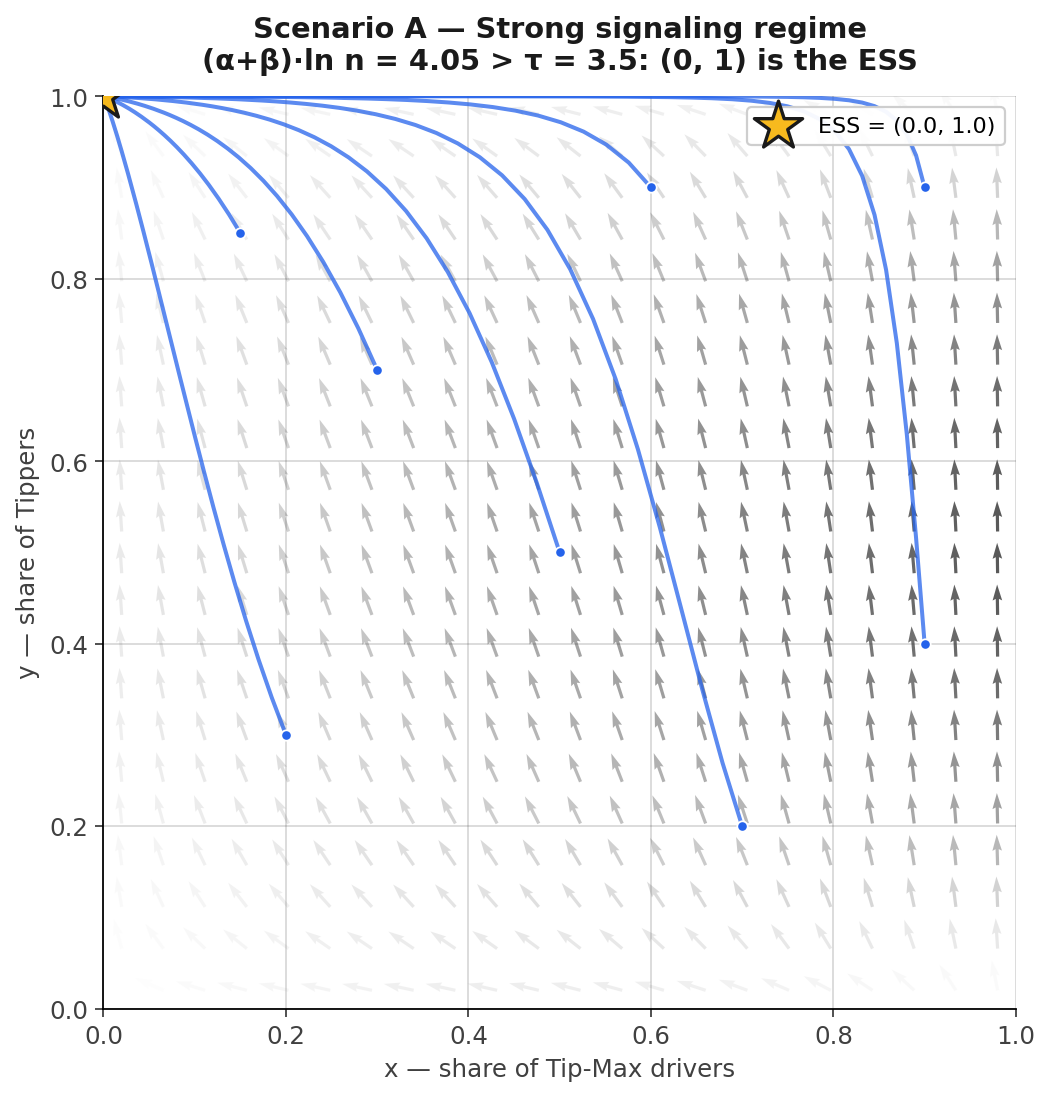
\includegraphics[width=0.6\textwidth]{figures/fig2_phase_cooperative.png}
\caption{Strong-signaling regime. Background arrows represent the velocity field of the replicator dynamics; blue curves are sample trajectories from different initial conditions. The indifference threshold $x^*$ is negative and falls outside the unit interval, so tipping pays for every starting point. All trajectories converge to $(0, 1)$.}\label{fig:strong}
\end{figure}

Figure~\ref{fig:strong} is an example of a strong signaling regime. The arrows in the background represent the velocity field of the replicator dynamics, and the blue curves are sample trajectories starting from different initial conditions. Tipping pays for every starting point. Because the indifference threshold is negative here and outside the range, there is no attainable point where a rider might change their strategy. Even if every driver is meter-maxing, the social reward $(\alpha+\beta)\ln(n)$ is so strong that it overcomes the cost of the tip. The driver payoff is still the same, $-m$, which drags $x$ to $0$, but passenger dynamics push $y$ upward because of the strong social signaling. This leads to every trajectory converging at $(0, 1)$.

\begin{figure}[h]
\centering
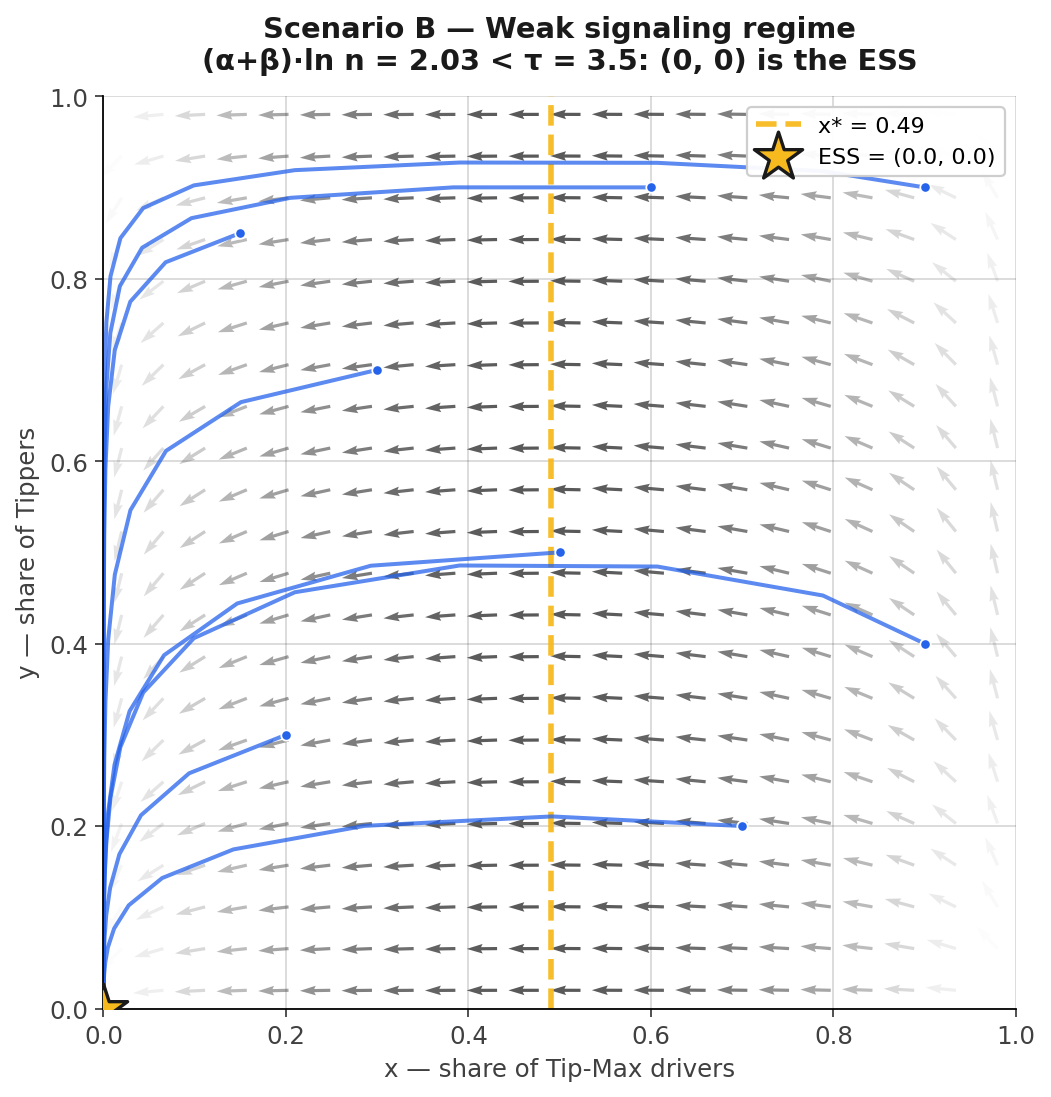
\includegraphics[width=0.6\textwidth]{figures/fig3_phase_collapse.png}
\caption{Weak-signaling regime. The threshold $x^* \approx 0.49$ is visible as the dashed yellow line. Trajectories above the threshold initially rise in $y$ while $x$ falls, but once they cross the threshold the passenger best response flips and $y$ collapses. All trajectories converge to $(0, 0)$.}\label{fig:weak}
\end{figure}

Figure~\ref{fig:weak} is an example of a weak signaling regime. This is the scenario where $(\alpha+\beta)\ln(n)$ is less than $\tau$. Now the point $x^*$ shifts toward the interior---in this case to $0.49$, represented by the yellow dashed line. The dynamics here are more nuanced: above $x^*$, there are enough efficient drivers that the expected social signaling reward from tipping still outweighs the cost of the tip, but below that point, the passenger's payoff flips sign, reflecting how non-tipping dominates. Trajectories that start above the threshold initially rise in $y$ even while $x$ falls, but when they hit the threshold, the passengers' response flips and $y$ crashes. Now all trajectories converge to $(0, 0)$: a full norm collapse, with no one tipping and no one driving efficiently.

Given that the model for the weak regime predicts full collapse to $(0, 0)$, this is what NYC tipping culture would look like if social signaling weakened. However, it is important to flag that our data tip rates hold near 95\%. This gap between prediction and observation is informative: real-world tipping in this regime would only persist because of external nudges that our basic model doesn't capture. Examples of these nudges include default 20/25/30\% buttons on in-cab payment screens, driver ratings, and social pressure from other passengers~\cite{haggag2014}. It is these mechanisms that keep the system off the $(0, 0)$ attractor predicted by our model.

\subsection{Equilibrium classification: Nash and ESS}\label{sec:ess}

\begin{table}[h]
\caption{Nash and ESS classification of the four corner equilibria. The cooperative outcome $(1, 1)$ is never evolutionarily stable. $(0, 0)$ and $(0, 1)$ are each ESS in mutually exclusive parameter regimes separated by the phase transition $(\alpha+\beta)\ln(n) = \tau$.}\label{tab:ess}
\begin{tabular}{@{}llcc@{}}
\toprule
Equilibrium & Description & Nash? & ESS? \\
\midrule
$(0, 0)$ & All MM, no tipping & Iff $(\alpha+\beta)\ln(n) < \tau$ & Same \\
$(1, 1)$ & All TM, all tip & No & No \\
$(0, 1)$ & All MM, all tip (norm-driven) & Iff $(\alpha+\beta)\ln(n) > \tau$ & Same \\
$(1, 0)$ & All TM, no tipping & No & No \\
\botrule
\end{tabular}
\end{table}

Table~\ref{tab:ess} summarizes the Nash and ESS status of each corner equilibrium of the strategy space. The cooperative outcome of efficient drivers and tippers is never an ESS because meter-maxing always invades, given that $\Delta f_{\mathrm{driver}} = -m$ is a constant and is hence unaffected by what the rider does. This reasoning applies to why $(1, 0)$ is also not a Nash equilibrium. As long as Meter-Max drivers gain anything positive from extending trips, the cooperative norm will always fail the ESS test. The cooperative outcome is therefore not merely fragile, but unattainable through reciprocity alone, with MM invading for as long as $m > 0$.

As illustrated in Figure~\ref{fig:weak}, all-MM with no tipping is Nash \emph{and} ESS only when signaling is weak, because $x$ collapses and drags $y$ down too once it falls below $x^*$. However, as shown in Figure~\ref{fig:strong}, when signaling is strong, tipping persists because the social signaling benefit $(\alpha+\beta)\ln(n)$ is greater than the tip cost $\tau$. Tipping then survives independent of what strategy the driver picks, making $(0, 1)$ a norm-driven ESS. This sets up our policy lever: strengthen signaling to stabilize tipping; weaken it and the norm collapses.

\subsection{Effect of the 2025 Congestion Fee}\label{sec:congestion}
On January 5, 2025, New York City instituted a flat \$1.50 congestion fee on trips entering the central business district. We use this policy as a natural experiment to analyze how drivers and riders respond to an actual change in their payoff parameters. Under the new congestion fee, drivers no longer need to extend trips to capture that extra revenue because it is now charged automatically.

\begin{figure}[h]
\centering
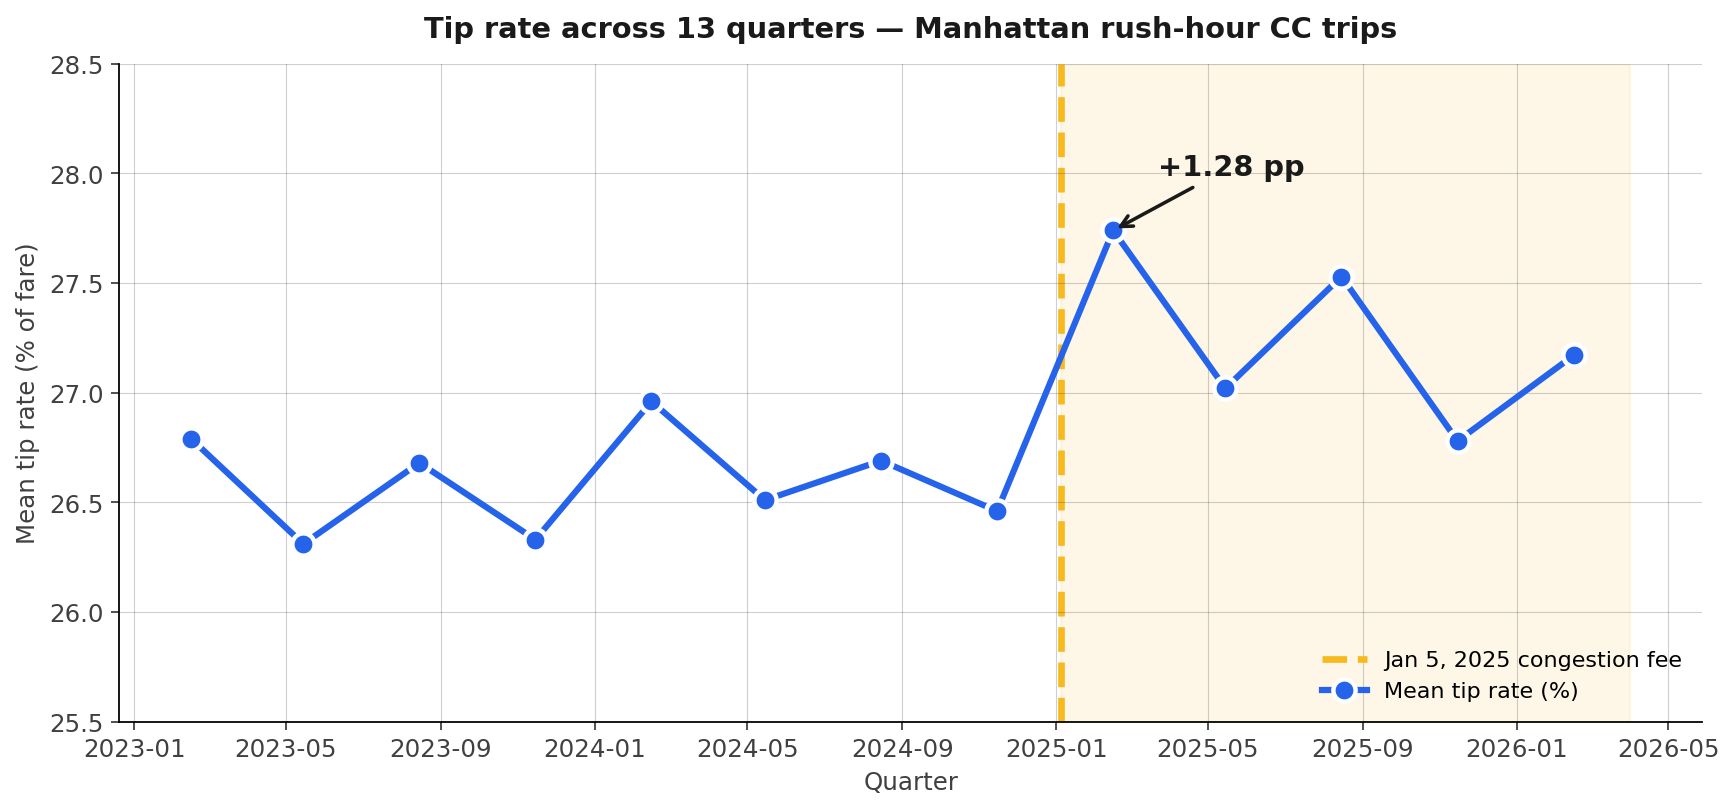
\includegraphics[width=0.9\textwidth]{figures/fig1_empirical_trajectory.png}
\caption{Mean credit-card tip rate across 13 quarterly snapshots, February 2023 through February 2026. The January 5, 2025 NYC congestion fee is marked; the +1.28~percentage-point jump from November 2024 to February 2025 is consistent with the model's prediction that compressing $m$ shifts the equilibrium toward more cooperative outcomes.}\label{fig:trajectory}
\end{figure}

Figure~\ref{fig:trajectory} plots the mean credit-card tip rate across the 13 quarters we looked at, with the congestion fee implementation date marked. From the graph, average tipping rates were stable at around 26.5\% through 2023 and 2024. After the congestion pricing fee was implemented, average tip rates increased by about 1.28 percentage points in the quarter following the fee and stayed consistently elevated afterward.

Considering our model, our estimate of $m$ fell substantially over the same interval, specifically from \$5.04 in November 2024 to \$3.46 in February 2025. The flat congestion fee means there are smaller opportunities for discretionary meter-maximizing behavior, which lowers the $m$ payoff in our model. Our model interprets this compression in $m$ as pushing the equilibrium dynamics toward more cooperative outcomes.

An additional key point worth noting in Figure~\ref{fig:trajectory} is that $m$ exceeds $\tau$ in every quarter, meaning that the meter bonus consistently exceeds the tip reward and thus confirms that the cooperative outcome $(1, 1)$ cannot be sustained. However, observed tip incidence holds near 95\% throughout, despite the model's prediction of the driver population drifting toward all Meter-Max. We can therefore conclude that NYC sits in the strong-signaling regime at the $(0, 1)$ equilibrium. Ultimately, the congestion fee's compression of $m$ changes the path toward this equilibrium through slower driver defection toward MM, giving the reciprocity channel more time to operate and reinforce the tipping norm. This finding is consistent with our model predictions and the observed 1.28~percentage-point jump.

%%%%%%%%%%%%%%%%%%%%%%%%%%%%%%%%%%%%%%%%%%%%%%%%%%%%%%%%%%%%%%%%%%%%%%%%%%%%%%
\section{Discussion}\label{sec:discussion}
%%%%%%%%%%%%%%%%%%%%%%%%%%%%%%%%%%%%%%%%%%%%%%%%%%%%%%%%%%%%%%%%%%%%%%%%%%%%%%

\subsection{Summary of contributions}\label{sec:contributions}
This paper formalizes taxi tipping as a two-population evolutionary game and derives the conditions under which tipping collapses or survives as a population-level norm. Our central contribution is demonstrating that the cooperative outcome---efficient drivers and tipping passengers---can never be an evolutionarily stable strategy. Meter-Max strictly dominates Tip-Max for drivers at every point in the strategy space. This is what separates our framework from a simply game-theoretic one to an evolutionary one. We are not asking whether cooperation is a Nash equilibrium in a one-shot interaction, but instead whether, over time, it can resist invasion and persist across a population of adapting agents. We can see that it cannot, at least not through reciprocity alone.

Social signaling is what sustains tipping in the real world according to our model. The phase transition at $(\alpha+\beta)\ln(n) = \tau$ divides the system into two qualitatively different regimes. In the strong-signaling regime, $(0, 1)$ is the ESS: all drivers meter-max, yet all passengers tip because the social cost of not tipping exceeds the monetary savings. In the weak-signaling regime, the system collapses entirely to $(0, 0)$. The natural congestion pricing experiment supports this: the compression of $m$ from \$5.04 to \$3.46 following the January 2025 fee corresponds directly to the observed 1.28~percentage-point increase in tip rates, which is consistent with equilibrium dynamics shifting toward more cooperative outcomes.

\subsection{Broader implications}\label{sec:broader}
Our findings can speak to an even bigger question within the social sciences: when do informal norms substitute for formal contracts, and when can they collapse? We have provided a concrete mechanism through our model that determines whether a norm can be self-sustaining or needs external scaffolding to survive. This is relevant to any gig-economy setting where workers and clients interact without binding contracts. Settings such as food delivery, freelance platforms, and peer-to-peer services all feature asymmetric information, voluntary compensation, and reputational dynamics that shape behavior. The EGT framework developed here can be applied directly to these settings.

Speaking of urban policy, these findings suggest things like transparency and default settings are doing much more than encouraging certain behaviors---they are helping the system not fail. The automatic 20/25/30\% tip options on the payment screens~\cite{haggag2014}, driver rating systems, and clear fare information help strengthen social expectations. These are not optional design features but rather essential parts of the system.

\subsection{Limitations}\label{sec:limitations}
Several limitations should be noted within our model. The model utilizes binary strategies where drivers either Tip-Max or Meter-Max, and passengers either tip or do not. This is not realistic, because real behavior is continuous: drivers choose how much to deviate from the optimal route and passengers can choose how much to tip. A continuous-strategy extension would better capture the marginal incentives. Second, replicator dynamics assume a well-mixed population where any driver can be matched with any passenger. However, matching is not random but rather shaped by neighborhood, time of day, driver reputation, and app algorithm, which introduce network structures that our model does not take into account. Our data only covers credit-card-paying passengers, meaning that we ignore cash tips entirely. Lastly, the key parameters---$m$, $s_0$, $\alpha$, and $\beta$---are estimated through proxies rather than directly observed. We have not conducted a formal sensitivity analysis to test how much our conclusions would change if these values were different.

\subsection{Future directions}\label{sec:future}
Three extensions stand out as the most promising. First, replacing the deterministic replicator with a Moran process would allow for finite-population effects and drift, which matter when social groups are small. Second, extending the model to rideshare platforms such as Lyft and Uber would incorporate driver rating systems, algorithmic dispatch, and enforcement mechanisms that interact with the informal norm. Finally, the phase transition result---that tipping survival depends on crossing a single threshold in social signaling strength---invites empirical testing. An experiment that varies passenger group size or default tip options could help determine where real New York City rides fall in relation to the $x^*$ threshold, and whether these changes can consistently move the system from one outcome to another.

\bibliography{refs}

\end{document}
